\newacronym{vtk}{VTK}{visualization toolkit}

In this section the methods used to accomplish the aims of the application are presented. The sections are ordered after the workflow the user has to perform. Not only the methods which are really used in the resulting application will be described also alternative approaches which may have not found their way into the final solution will be presented. It will also be described why and how we have decided which approaches fit best for the solution.

\section{Application overview}

In the first section the aim is to give the reader an overview of the presented methods. Figure \ref{fig:methodsOverview} shows the workflow of the application. The first step is loading of the data. This step can be very complex because it highly depends on the format the data are provided. In case of ultrasound data originating from an clinical investigation or already registered data representing the whole fetus, the data format might be \gls{dicom}. Another possibility would be to provide the data using a *.raw format which only include the data itself and no surrounding information which e.g. \gls{dicom} includes. The *.raw format might come along with a *.mhd file which is also called the MetaHeader and represents meta information about the data included in the *.raw file. The data might also come in various other formats and therefore there might be some restrictions. Thinking about loading data the usage of the tools MeVisLab \cite{AGMeVisLab} or 3D Slicer \cite{Slicer3DSlicer, Fedorov20123DNetwork} is endorsed. Both software solutions are publicly available, open source and for free.\newline

\begin{figure}
    \centering
	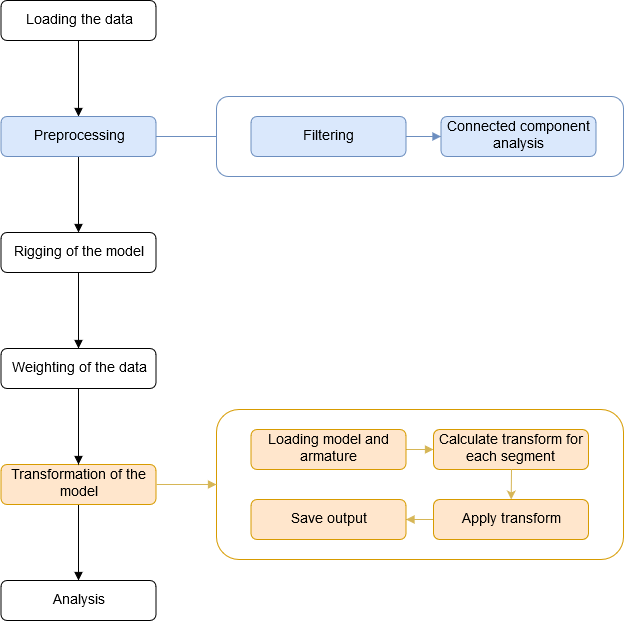
\includegraphics[width=15cm]{content/images/MethodsOverview}
	\caption{The application overview represents the pipeline that has to be performed in order to result in a T-pose fetal representation.} 
	\label{fig:methodsOverview}
\end{figure}

The next step is called preprocessing and depends highly on the input data. The data can be visualized in different applications like MeVisLab or 3D Slicer. The preprocessing pipeline used in this thesis includes a threshold processing be able to distinguish between background data and the data belonging to the fetus. The next step is to calculate the larges connected component in the data and get rid of all other information in the dataset. The output of this step is a volume only holding information about the fetus.\newline

One of the larger and also very important steps is to rig the data. This step can be performed in lots of different ways. One solution might be to use the Bender software which is based on 3D Slicer and the paper about it has been written by Finet et.al. \cite{Finet2014Bender:Morphing}. Bender is also an open source program which includes various modules for model posing and morphing. One model is called armature and can be used to create and place an armature in a model.\newline

The next step in the pipeline describes the weighting or skinning of the data. This processing step is used to calculate the contribution of different segments of the armature to the input data namely the volumetric data of the fetus. The output of this processing step is a volume which includes the mapping for each voxel to one of the armature segments. This step might also be performed using Bender \cite{Finet2014Bender:Morphing}. In Bender the module VolumeSkinning shall be used which needs as input the armature and the volume. The result will be just the described one.\newline

The most unique and novel part of the pipeline is the transformation of the model. This processing step is used to actually transform the data. The transformation is performed automatically. As an import the armature and the volumetric data is required. The volume has to be weighted and each segment of the armature has to be mapped to some voxels. The transformation calculates the needed transformations of each segment in respect to the adjacent ones, resulting in a fetus model at a T-position. As represented in the overview Figure \ref{fig:methodsOverview} with a dashed line the transformation of the model might result in a feedback loop back to the rigging. The user might want to reset some joint positions in order to get a more realistic and representative result in the end. The transformation will be described in greater detail in the section \ref{sec:transformation}. The output of the transformation can be in different file formats but it is recommended to choose a well known form in order enable the analysis to be performed in different consumer products.\newline

The last step of the pipeline is named analysis and has the aim to gather insight in the now transformed data. A part of the analysis step could be automatically done e.g. some measurements like the finger to finger span or the head to toe length. The user gets new insights in this module and is be able to interactively view the now unfolded data. Taking measurements like specific circumferences or lengths like the femur length for example should be possible. This module can be very user specific because it depends on the preferences of the user and which modules they would like to use. Having a nice rendering of the volumetric data might also be interesting where approaches using the \gls{gpu} might be interesting. One example is the GVDB library by NVIDIA which is particularly written for voxel visualization \cite{Hoetzlein2016}.

\section{Loading the data}

Loading the medical or phantom data is a step which occurs not only once during the processing of the data. Some processing steps of the pipeline may not be implemented using the same system and therefore data exchange namely loading and generating output is essential. Loading of the data somehow differs between the modalities used. In this section the loading steps which are used in this thesis are described.\newline

\subsection{MeVisLab}

The first loading step is performed in MeVisLab \cite{AGMeVisLab}. MeVisLab is a tool which consists of a large amount of modules which the user can choose. Certainly there are many different modules to load data. In this thesis two can be used namely the $ImageLoad$ or the $LoadAny$ module. The $ImageLoad$ module and the corresponding properties can be seen in Figure \ref{fig:meImageLoad}. The $ImageLoad$ module is used to examine *.raw data but the user has to define the spatial resolution and the data type which is included in the *.raw file.

\begin{figure} [!htb]
    \centering
	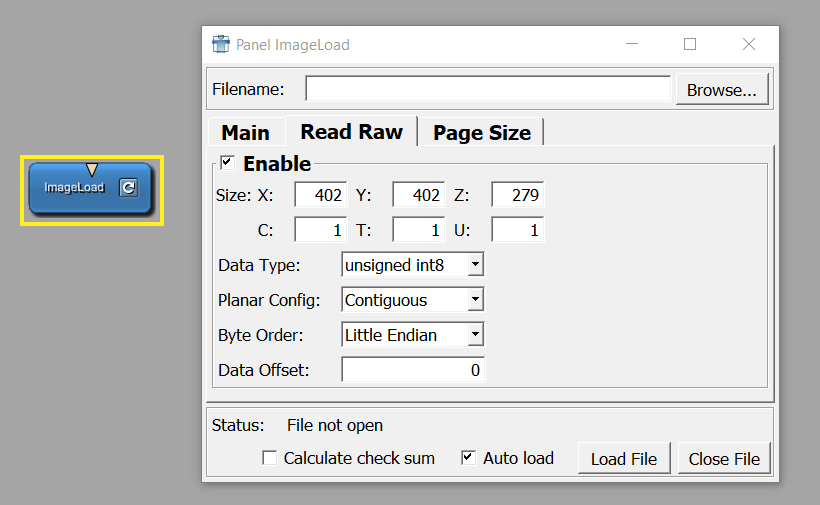
\includegraphics[width=10cm]{content/images/meImageLoad}
	\caption{The screenshot shows the $ImageLoad$ module and the corresponding settings where the user has to define the resolution of the *.raw file and the data type.} 
	\label{fig:meImageLoad}
\end{figure}

If the data is present in a *.mhd file format one might just use the $LoadAny$ module. This module has the benefit that the user does not have to apply any settings but the file has to support being loaded. A *.raw file might not be loadable because the module does not have any contextual information included.

\begin{figure} [!htb]
    \centering
	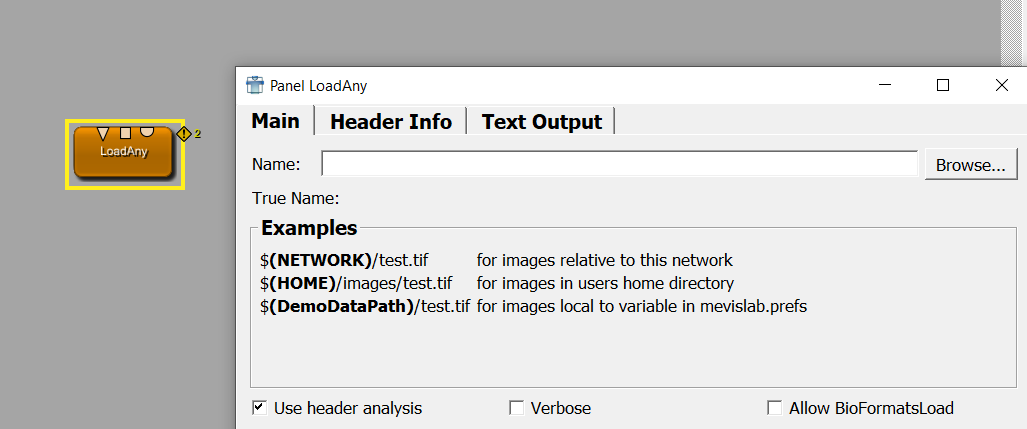
\includegraphics[width=12cm]{content/images/meLoadAny}
	\caption{The $LoadAny$ module of MeVisLab which can be used to load e.g. *.mhd files along with the corresponding *.raw file without having to set any properties.} 
	\label{fig:meLoadAny}
\end{figure}

\newpage
\subsection{3D Slicer and Bender}

3D Slicer \cite{Slicer3DSlicer,Fedorov20123DNetwork} as well as Bender \cite{Finet2014Bender:Morphing} which is a 3D Slicer based application do also provide to load the medical data and this option is used during this processing steps. Loading data is quite simple using those programs. Loading data in 3D Slicer is performed by clicking on the button highlighted in the Figure \ref{fig:slcLoad} and in Bender by clicking the button in Figure \ref{fig:bendLoad}. Both loading steps are simply performed by selecting the file to load, unfortunately both applicaions do not support loading files in *.raw format. The data is automatically available for visualization and further processing in the software.

\begin{figure} [!htb]
    \centering
	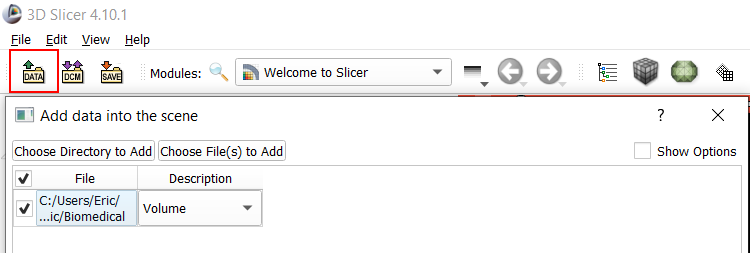
\includegraphics[width=12cm]{content/images/slcLoad}
	\caption{Loading of data in to the 3D Slicer program.} 
	\label{fig:slcLoad}
\end{figure}

\begin{figure} [!htb]
    \centering
	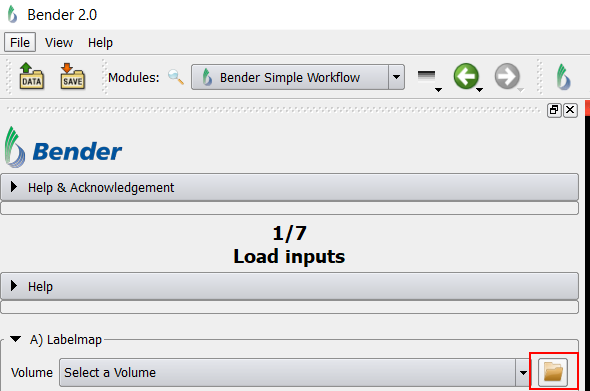
\includegraphics[width=8cm]{content/images/bendLoad}
	\caption{Loading data for being processed in Bender.} 
	\label{fig:bendLoad}
\end{figure}

\subsection{Phantom data generation}

When thinking about a transformation of ultrasound data to a specific position the question arises how the approach should be validated. There is no ground truth so to say if the found transformation is good or bad. Therefore in this thesis a phantom approach has been used. The phantom data represents a human in a T-pose. The model can be transformed into different fetus like poses using Blender \cite{Foundation2019Blender}. Blender enables the user to perform the rigging process and afterwards use the Pose option in order to generate different poses to be tested with the introduced workflow. The model used in this thesis has been found in the internet and is licensed by the Royalty Free License with allows all extended usages and can be fond here \cite{Squidifier2010DetailedMan}. It has to be mentioned that Blender works with a mesh and therefore surface representation of the \gls{3d} models and this data would not be loadable. Therefore a processing step has to be performed to generate a voxelized model out of the mesh.

\subsubsection{STL generation}

The first step towards a voxelized model representation of a mesh is to export the mesh in the *.stl format which is supported by Blender off the shelf. One only has to select the option export as stl and this step is already done.

\subsubsection{STL to image stack}

After having generated the *.stl file of the mesh model the next step is to convert it into an image stack. During the work on this thesis a public available python script has been used namely $stl-to-voxel$ \cite{Pederkoff2015Stl-to-voxel}. This pyhton script transforms the *.stl mash format in a stack of images which can be interpreted as voxel values. The transformation into an actual \gls{3d} volume file is done in the next step using another tool. The python scrip has to be run with the *.stl file and a folder as input. In then generates the images. It might be useful if the resolution is increased by altering one line of code in the file $stltovoxel.py$. The list line number 99 defines the resolution of the image in x and y axis. The default value is 100 and for the data used during this thesis 400 seemed to be an appropriate value. An example input and output situation of the script is shown in Figure \ref{fig:stlToVoxel}.

\begin{figure} [!htb]
    \centering
	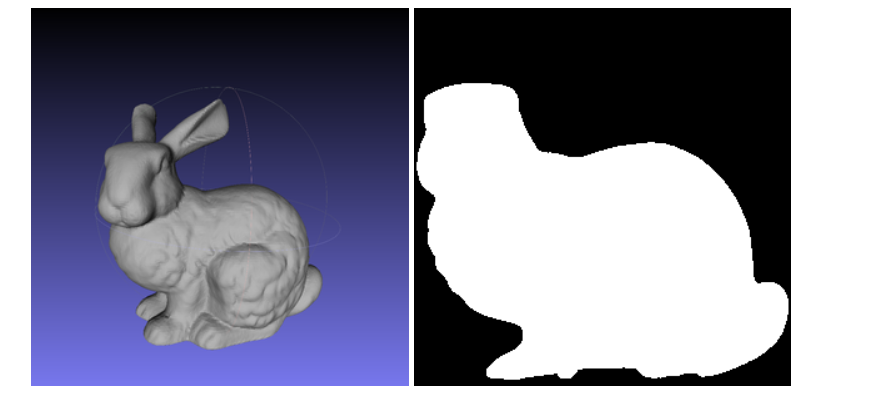
\includegraphics[width=14cm]{content/images/stlToVoxel}
	\caption{Example of the $stl-to-voxel$ python script showing the mesh representation on the left and one image of the image stack on the right.} 
	\label{fig:stlToVoxel}
\end{figure}

\newpage
\subsubsection{Convert image stack to *.raw file}

The last step in the phantom data generation is to convert the image stack given as an output form the $stl-to-voxel$ python script into an actual volumetric dataset. This step is performed using the tool ImageJ  \cite{Ecosystem2018ImageJ}. ImageJ is an open platform for scientific image analysis. The tool provides an import for the given image stack simply by selecting the option $File$ $Import$ and $Image Sequence$ and selecting the first image of the image stack. The *.raw file can be saved by selecting the option $Save As$ and $Raw Data$.

\newpage
\section{Preprocessing}

The preprocessing step depends as stated before highly on the data which has to be processed. In case of a fetal ultrasound investigation the data might be affected by artefacts and information which does not belong to the fetus. Cortes et.al. introduced in their paper a dataset of a phantom ultrasound investigation with artefacts included which may also arise in that way during a \gls{3d} fetal ultrasound investigation \cite{Cortes2016UltrasoundEvaluation}. In order to depict the preprocessing steps introduced in this section the publically available dataset of the authors will be used. The data example before the preprocessing can be seen in Figure \ref{fig:phantomFetusOr}.

\begin{figure} [!htb]
    \centering
	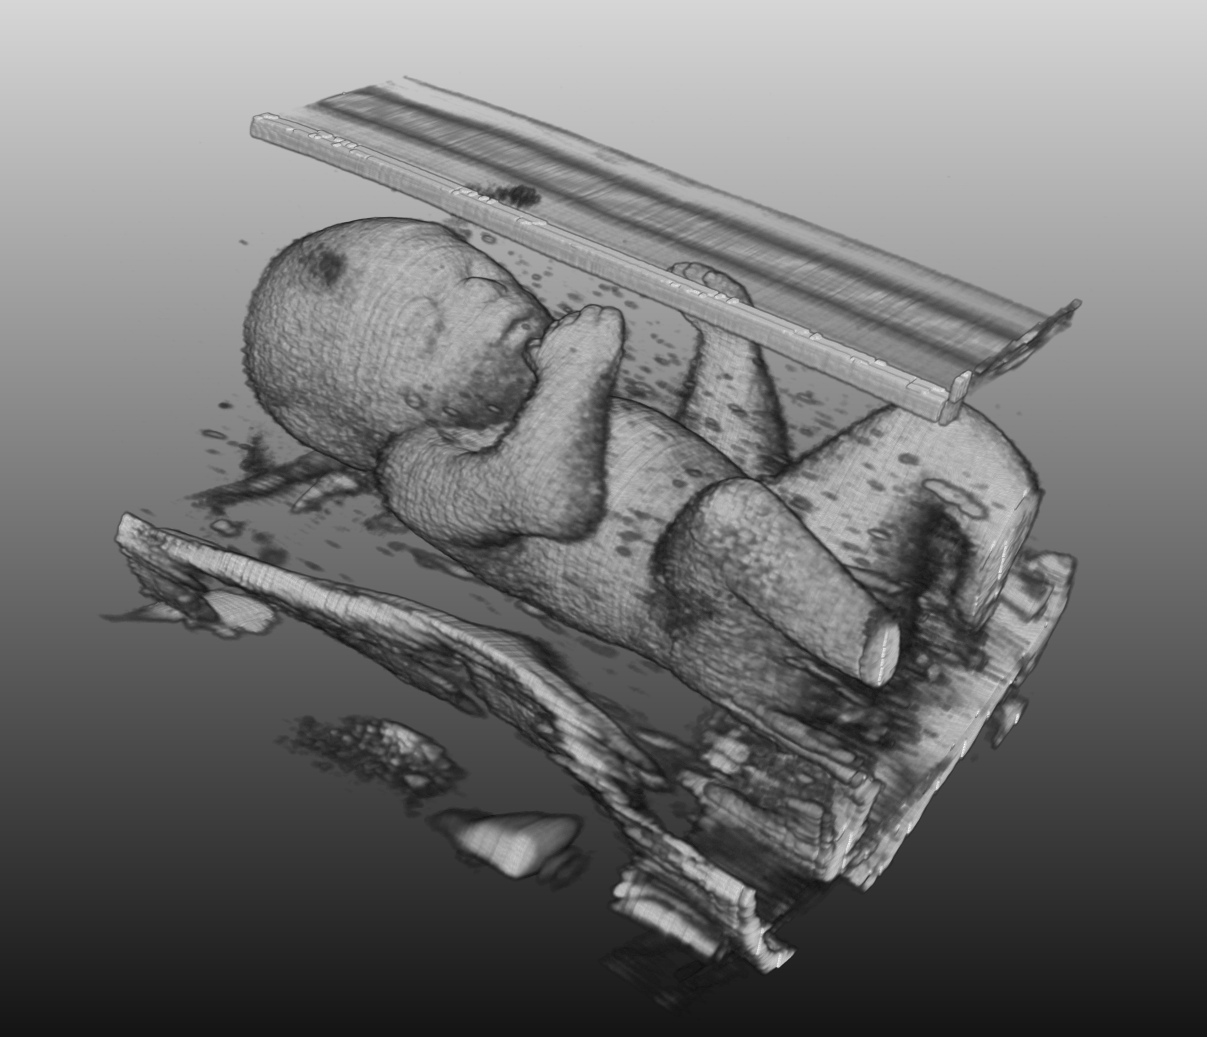
\includegraphics[width=8.5cm]{content/images/phantomFetusOr}
	\caption{The fetus phantom model data including arteficts which may also arise during a \gls{3d} fetal utlrasound investigation \cite{Cortes2016UltrasoundEvaluation}.} 
	\label{fig:phantomFetusOr}
\end{figure}

\newpage
\subsection{Filtering}

The first step is to apply a threshold. This operation is used to get rid of some of the artefacts in the data and to have a cleared view of the fetus. The module used in MeVisLab is called $Threshold$ and in the Figure \ref{fig:phantomFetusTh} a value of greater than 60 is used.

\begin{figure} [!htb]
    \centering
	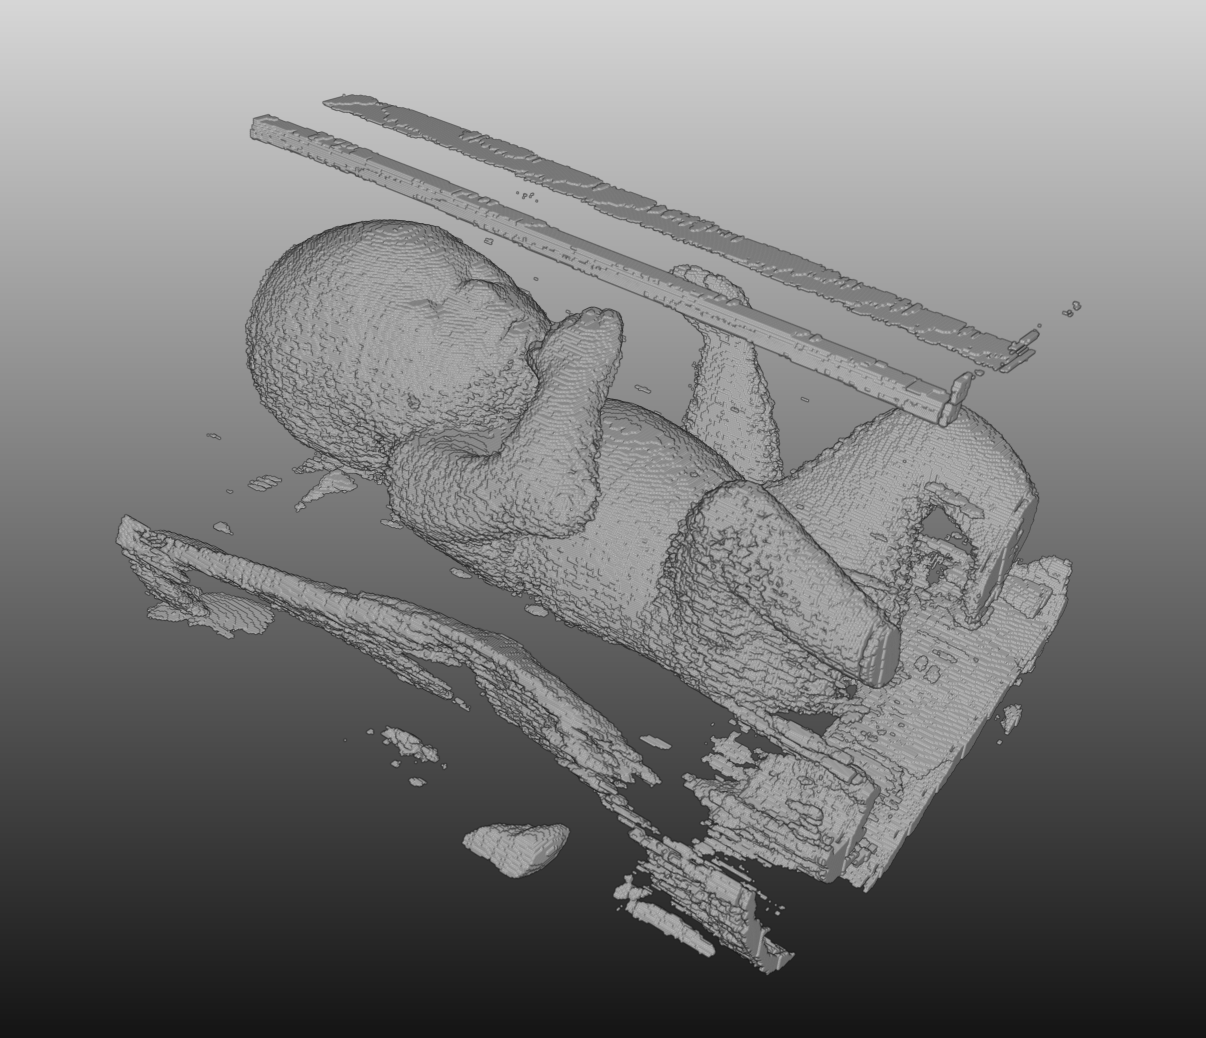
\includegraphics[width=8.5cm]{content/images/phantomFetusTh}
	\caption{The fetus phantom model after applying a threshold greater than 60.} 
	\label{fig:phantomFetusTh}
\end{figure}

\subsection{Connected component analysis}

The last step of the preprocessing pipeline is the so called largest connected component analysis. This step is used in order to get rid of all elements in the volumetric dataset, which are not connected to the fetus. It is defined that the fetus in the gathered ultrasound investigation data consists of one large component without any detached parts. The second thought is that in a fetus centered ultrasound investigation the fetus should of course be the largest component in the dataset. In order to calculate the largest connected component and filter the others three components are used namely $ComputeConnectedComponent$, $FilterConnectedComponents$ and $ConnectedComponentsToImage$. The first module takes the thresholded image data as an input and calculates the connected components. The second one is used to filter the components and search for the largest one by setting the $selectionMode$ to $Largest$. The last stated module finally converts the component back to image data which then can be visualized again. The result of this processing step can be seen in the following Figure \ref{fig:phantomFetusCCA}.

\begin{figure} [!htb]
    \centering
	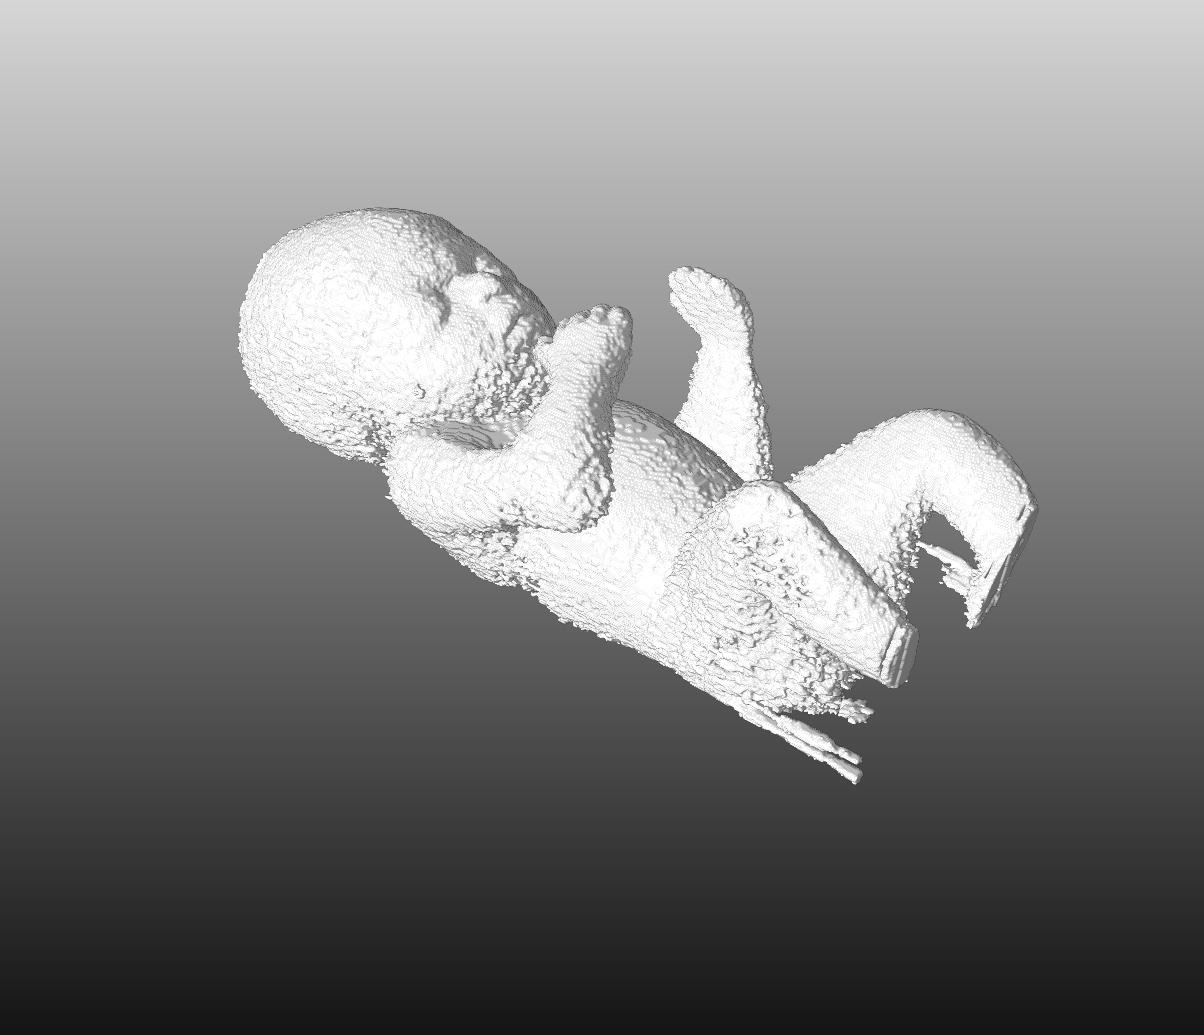
\includegraphics[width=8.5cm]{content/images/phantomFetusCCA}
	\caption{The fetus phantom model after applying a threshold greater than 60.} 
	\label{fig:phantomFetusCCA}
\end{figure}

\newpage
\section{Rigging of the model}\label{sct:rigging}

Rigging of \gls{3d} models can be done in many different ways, during this thesis the approach implemented by Bender \cite{Finet2014Bender:Morphing} has been used. The first step was to produce a template skeleton which is rather simple and does not provide too many segments that have to be included in the structure. When thinking of simplification a good tradeoff between losing details and having too less details has to be found. The Skeleton used in terms of this work is composed out of 20 segments and of 18 joints. Figure \ref{fig:Armature} shows a schematical representation of the produced armature. The representation of this armature in Bender can be seen in Figure \ref{fig:arm}.\newline

\subsection{Bender}
The rigging in Bender is done by simply dragging the skeleton piece by piece into the model. The \gls{3d} navigation has to be used in order to analyse if each part is correctly placed along each axis. The difficulty behind this approach is that in some cases the parts seem to be perfectly placed but when having a look in another representation the segments are not correct. The user has to check each segment along each axis and drag the segments until the place is correct along each axis. This procedure might seam tedeous and complex but unfortunately there have not been any known approaches to rig characters automatically that are already in a transformed position which differs completely from the known T-pose. Figure \ref{fig:rigging} represents the input of the rigging process and the result.

\begin{figure} [!htb]
    \centering
	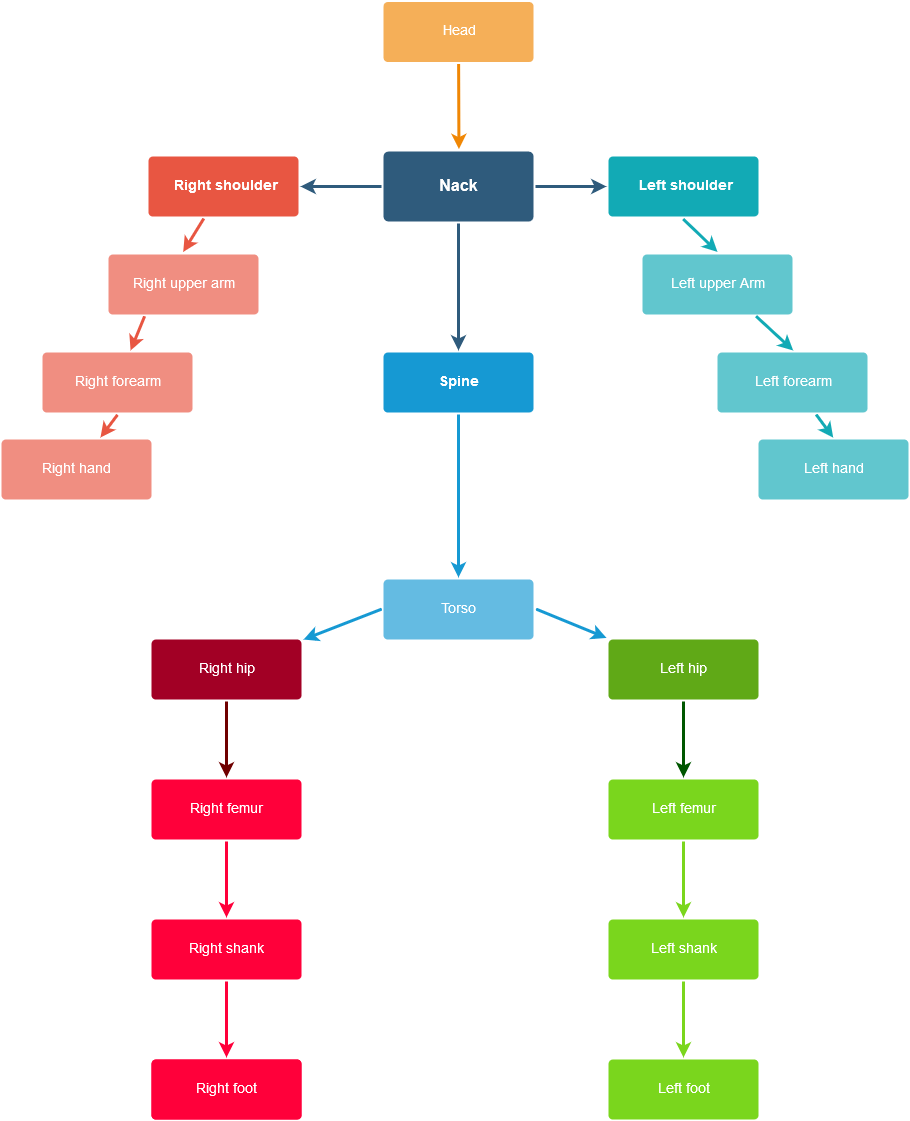
\includegraphics[width=14cm]{content/images/Armature}
	\caption{Schematical representation of the armature used in bender consisting of 20 segments and 18 joints.} 
	\label{fig:Armature}
\end{figure}

\begin{figure} [!htb]
    \centering
	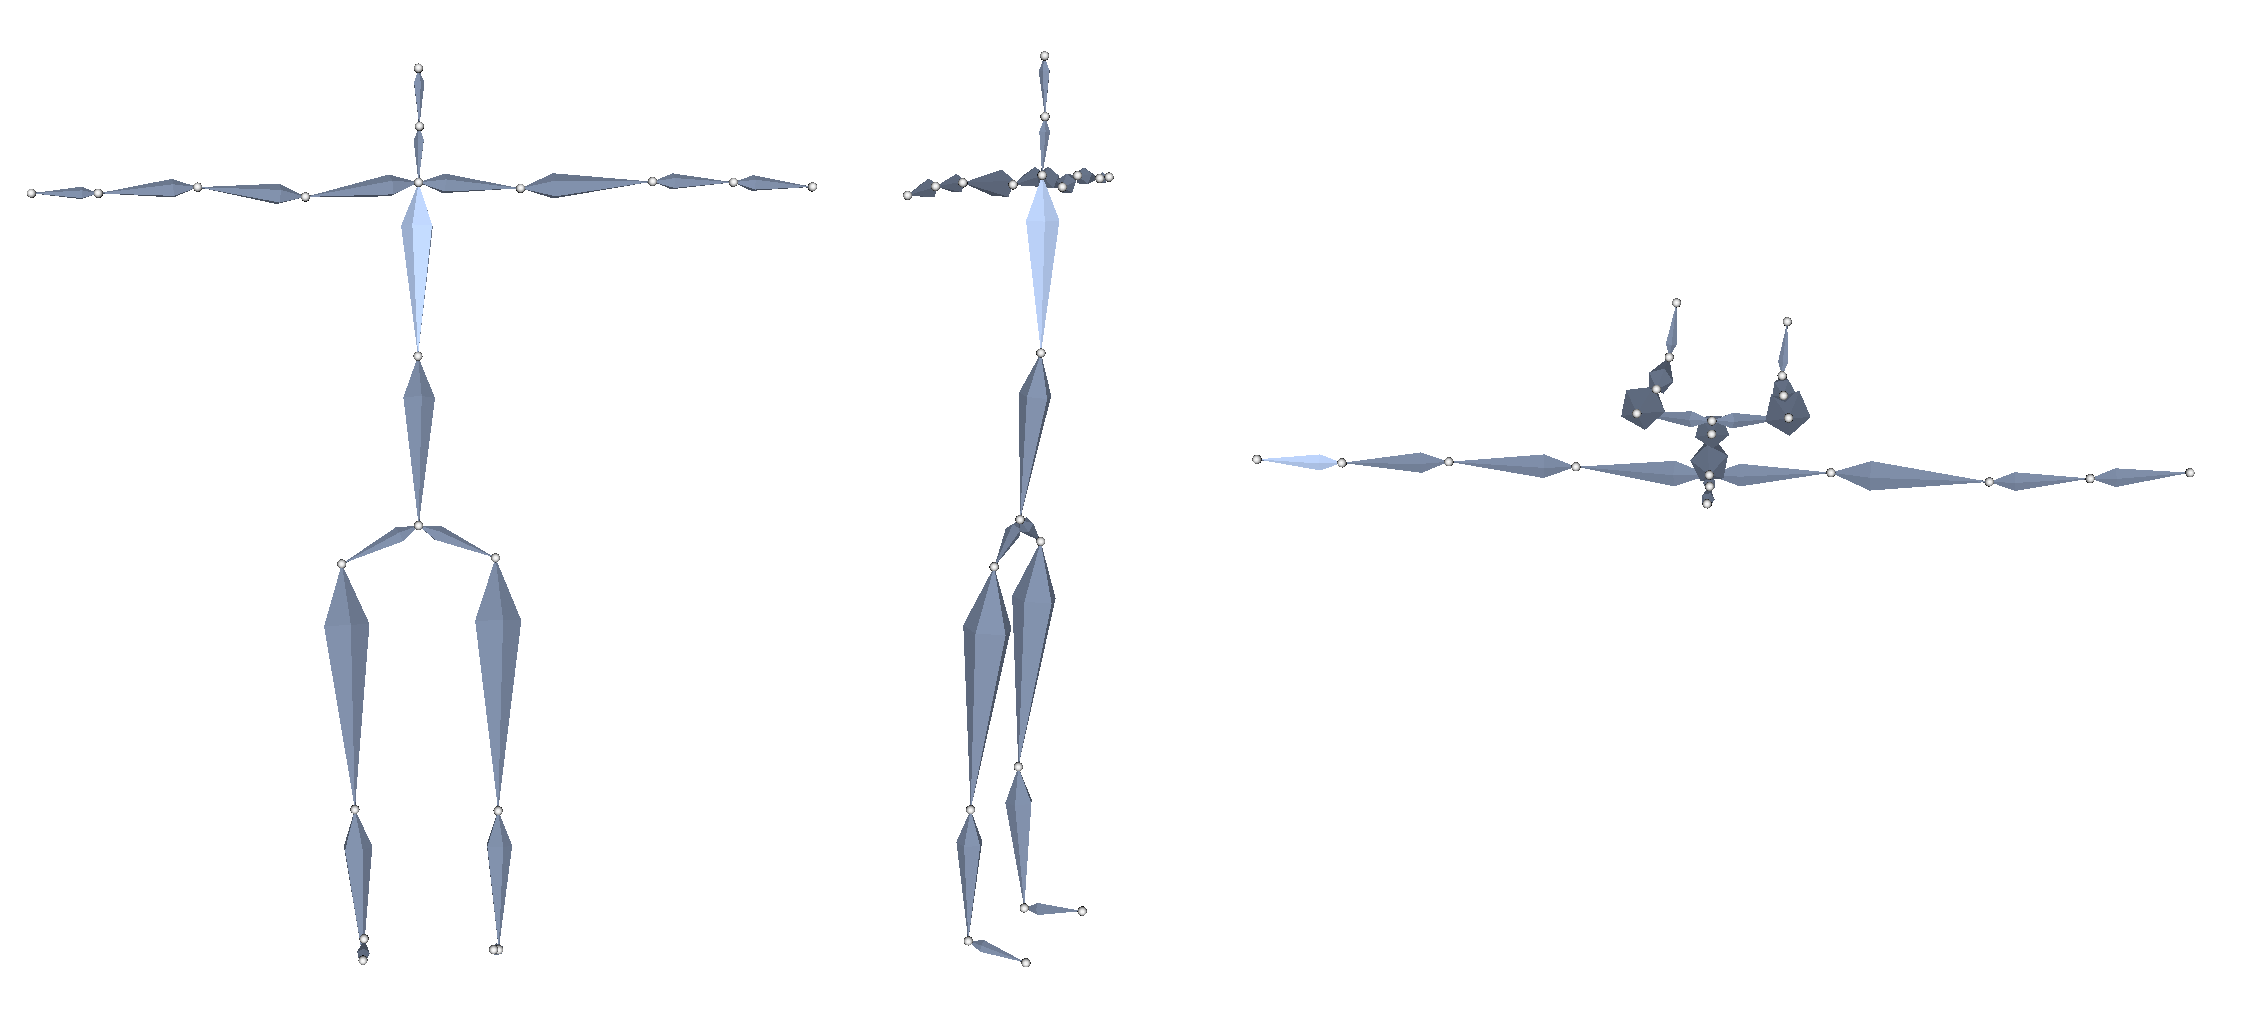
\includegraphics[width=15cm]{content/images/arm}
	\caption{Representation of the template armature in a T-position in Bender using a octohedronal representation} 
	\label{fig:arm}
\end{figure}

\begin{figure} [!htb]
    \centering
	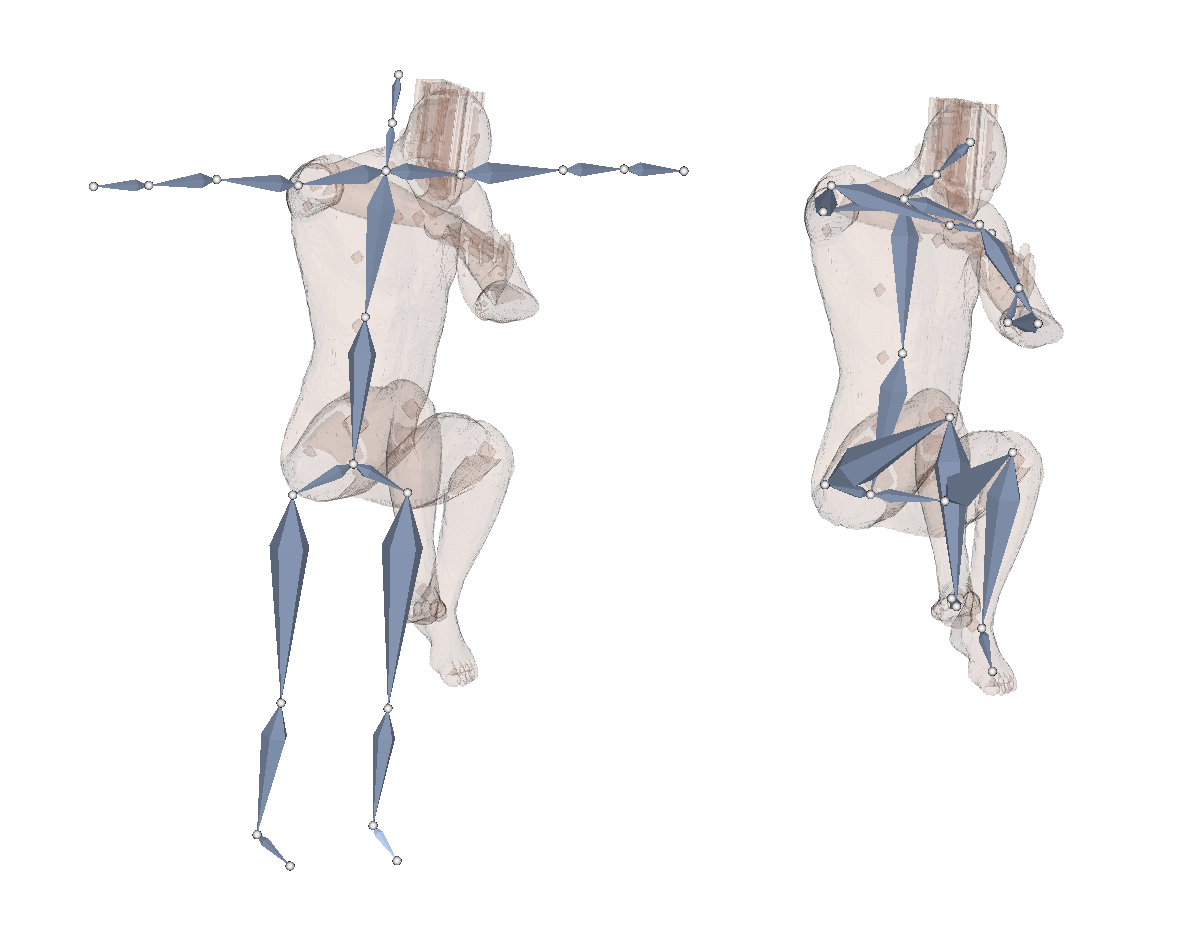
\includegraphics[width=12cm]{content/images/rigging}
	\caption{On the left side of the picture a phantom model of a man and the armature representation in Bender can be seen. The right image shows the result namely the armature perfectly in place.} 
	\label{fig:rigging}
\end{figure}

\newpage
\subsection{GPU based voxel visualization}

Another approach of rigging the data would be to implement a way to identify and work with keypoints of the model and automatically incorporate the armature. Therefore one approach might be to use a \gls{gpu} based approach to visualize and analyse the data. NVIDIA introduced in 2016 a \gls{gpu} based voxel database called GVDB which can be used as an efficient data structure for voxel visualization \cite{Hoetzlein2016}. Their approach is open source looked promising as a starting point for the tasks in this master thesis. First the visualization aspect has been analysed and worked out well. The example section of NVIDIA provided an out of the box loading algorithm which can be used in terms of *.raw data and the loading worked perfectly.\newline
In this work a simple and new approach has been introduced to select data based on a abstract representation of the voxel data. GVDB provides different abstraction levels which have been used in order to select parts of the voxelized model interactively using the three axis. The user had the option to move with the mouse and select a starting and an ending point along each axis to summarize six selections. The result would be a very simple selection process resulting in the selection of a specific part of the model which than would be highlighted. The selection process and the highlighted section of the data is depicted in Figure \ref{fig:gvdb}. The approach was unfortunately not used in the end because there was no option how to apply transformations to only parts of the model which would have been needed in order to transform the data to a T-pose.

\begin{figure} [!htb]
    \centering
	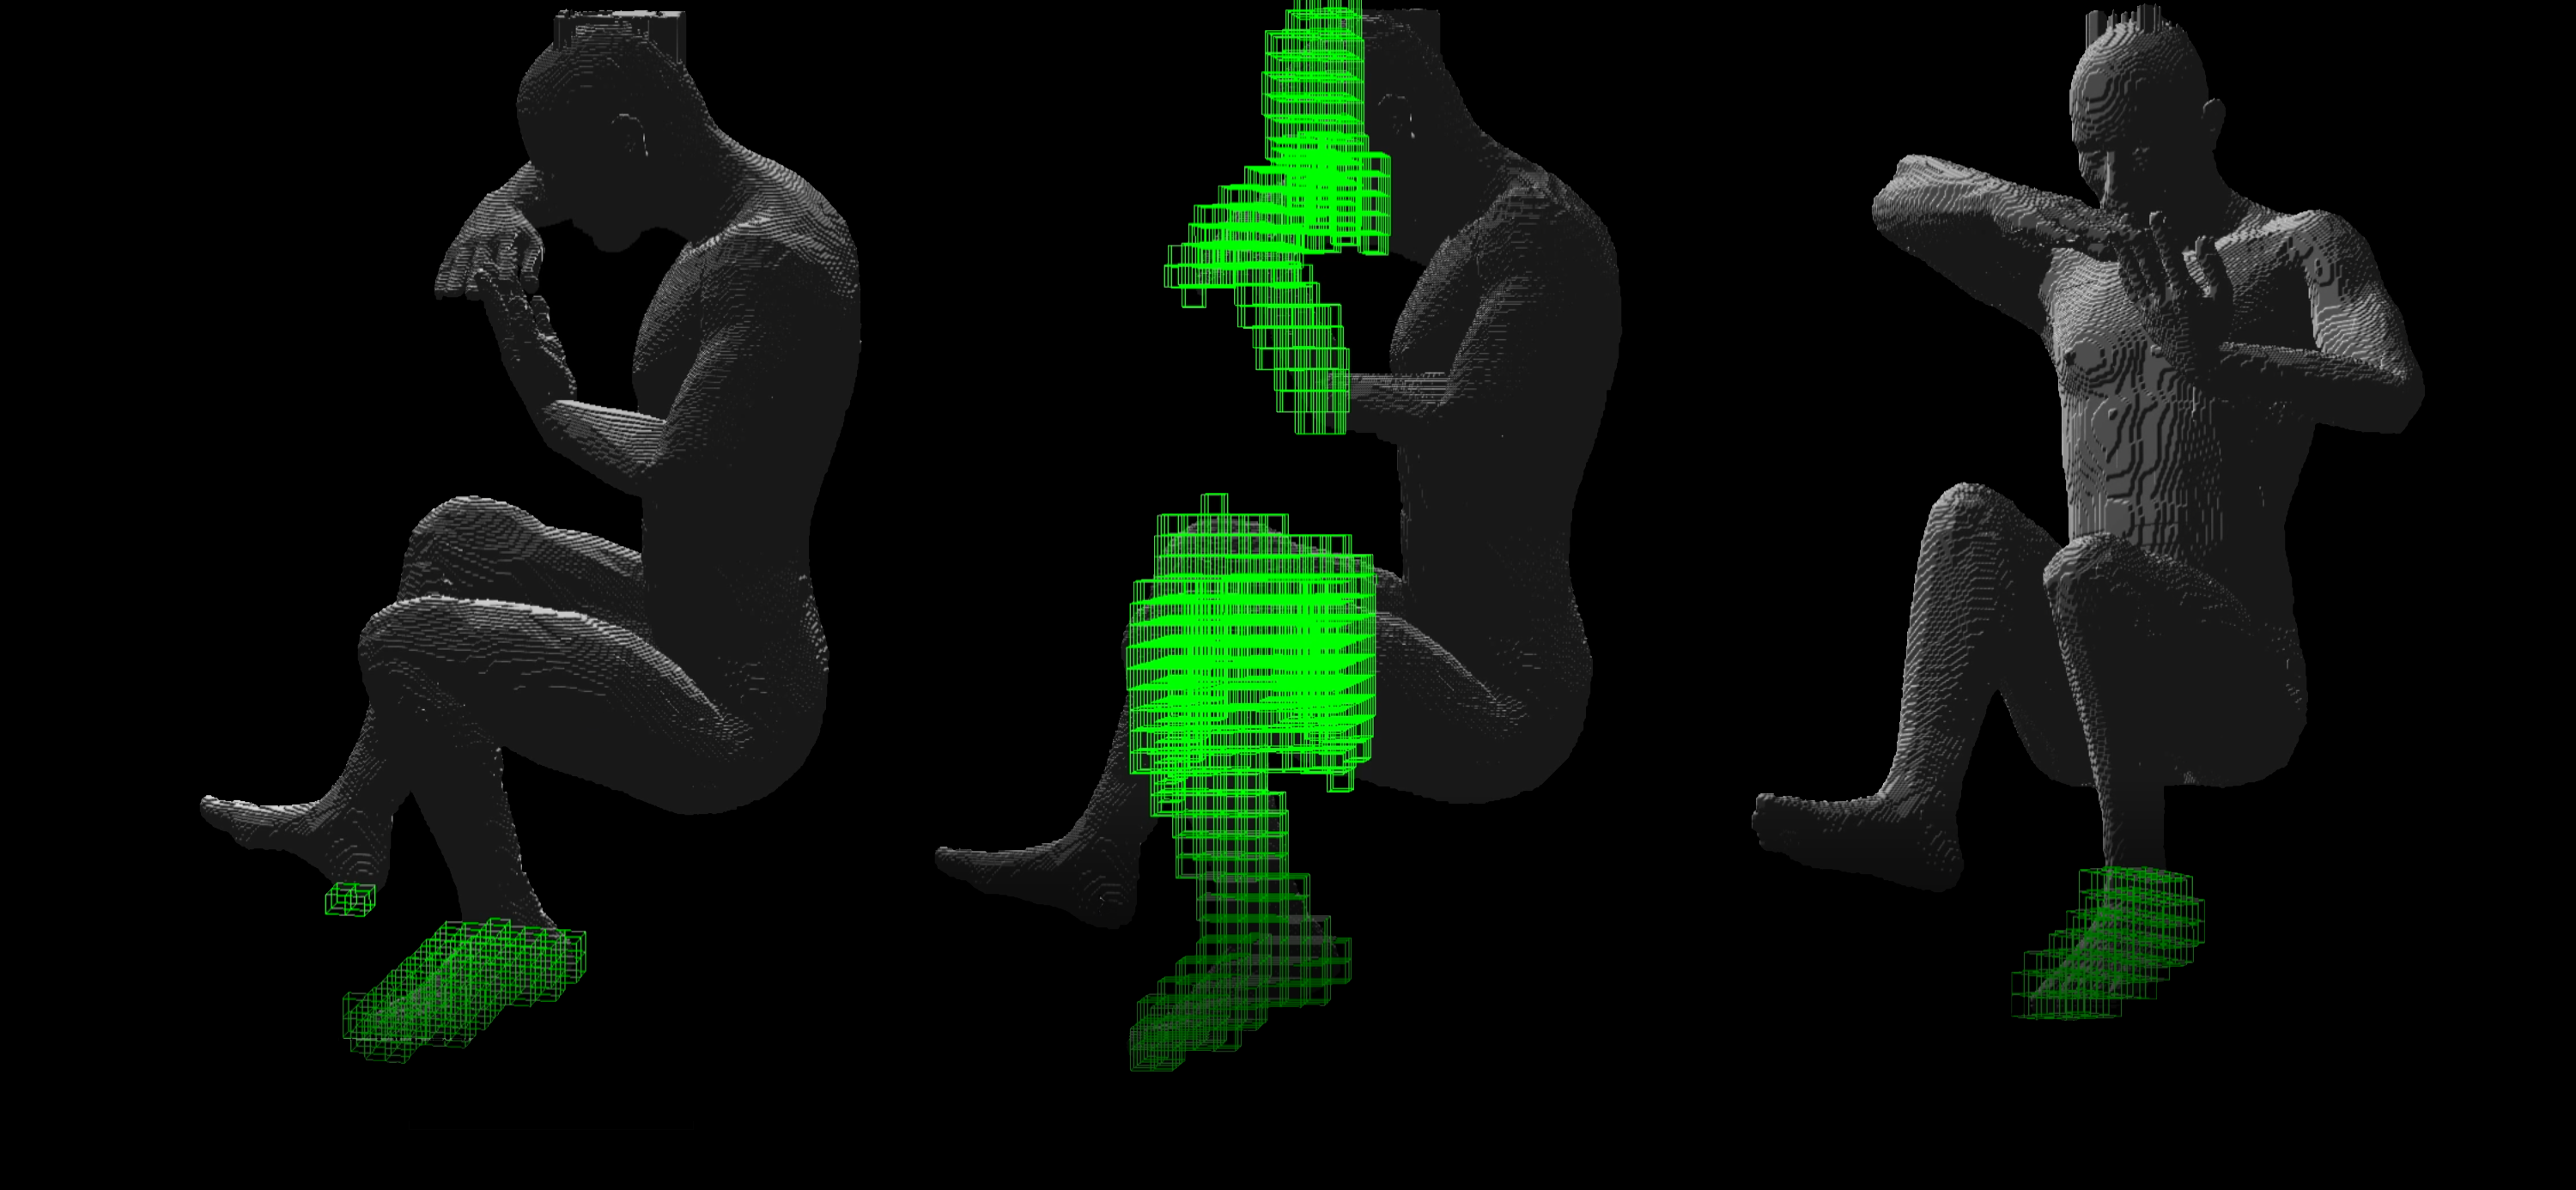
\includegraphics[width=14cm]{content/images/gvdb}
	\caption{The left and the middle image represent the selection process of the one keypoint in the data namely the left foot of the phantom. The right image shows the selected foot represented in green. The green boxes are a representation of the data on a higher level in the GVDB database.} 
	\label{fig:gvdb}
\end{figure}
\newpage
During the work on this master thesis different approaches have been tried to figure out how to automatically perform the rigging of the volumetric data. Unfortunately all approaches that have been tried did not deliver sufficient results. Although those attempts failed the results of them are stated in this section in order to explain and show what went wrong.

\subsection{Pinocchio}
The Pinocchio prototype introduced by Baran and Popovic is open source and available to download online \cite{Baran2007}. As stated in chapter \ref{ch:related} their approach need a watertight mesh as an input and will automatically calculate the armature which is somehow based on a predefined skeleton. In the paper about the automatic rigging and automation of \gls{3d} character the authors already mention that the discrete penalty functions used picture some assumptions which might lead to a unsatisfactory result when using their approach. Another downside of their algorithm is that it only works with mesh data and the data of fetal ultrasound investigations are normally given in voxel format. The transformation from the voxel data to a watertight mesh would lead to a loss of information and might not even be possible without human interaction. Although Shapiro et.al. introduced an algorithm based on the Pinocchio prototype which works with a voxel model as input. Unfortunately their implementation is not publicly available. The results when using the Pinocchio approach are depicted in Figure \ref{fig:PinocchioSkeleton}. The reason why this approach has not been progressed is that it seems that it will only work if the input data is somehow given in a standardized position.

\begin{figure} [!htb]
    \centering
	\includegraphics[width=7cm]{content/images/Pinocchio}
	\caption{Result of Pinocchio prototype applied to the man phantom model in its mesh representation.} 
	\label{fig:PinocchioSkeleton}
\end{figure}

\subsection{Skeletonization}
Another approach for the automatically rigging was to find a skeletonization representation of the data which may afterwards be mapped using joint mapping like introduced by Bharaj et.al. \cite{Bharaj2012}. This approach would need a curve skeleton as an input which perfectly represents the volume and is not somehow to complex. There are different approaches how to skeletonize a mesh but when working with voxels the selection is restricted. Altought two approaches have been tried. One is based on a Matlab toolbox called Volume Skeleton Toolbox. This toolbox provides different approaches for calculating the curve skeleton of volume data by thinning, distance field or potential field. When trying the approach with the distance matrix the result consisted of a huge amount of points. The potential field approach did not terminate and delivered a runtime exception and the thinning method somehow represented a skeleton but it was way to detailed. The result can be seen in Figure \ref{fig:skeleton}.\newline
It has also been tried to generate the Skeleton in MeVisLab using the $DtfSkeletonization$ module. The result of this approach is also depicted in Figure \ref{fig:skeleton}. It seams that there are some points of interest like the knee or other joints but it is also way to detailed and did not improve significantly when trying to use different settings in the module.

\begin{figure} [!htb]
    \centering
	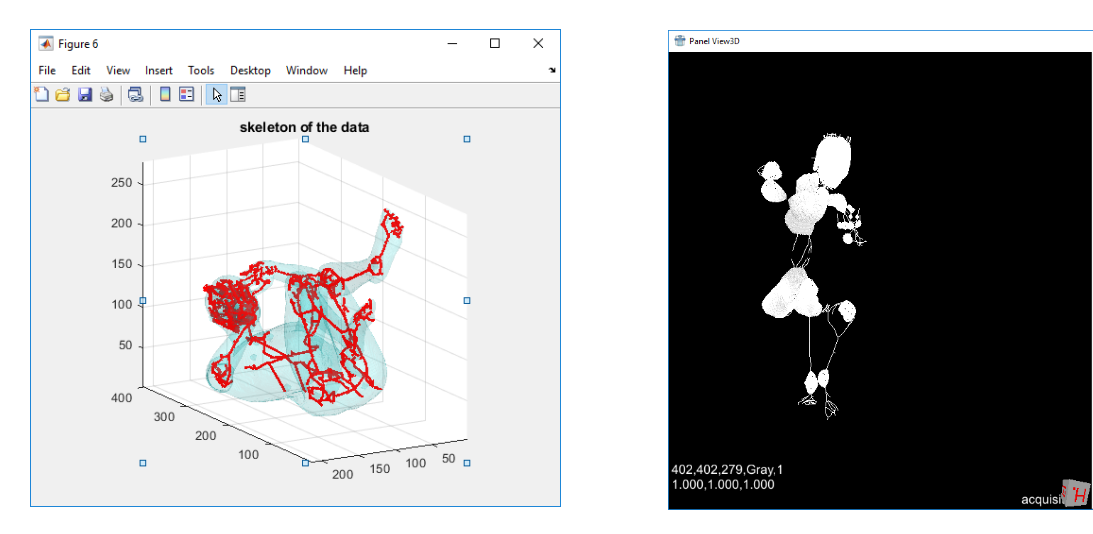
\includegraphics[width=15cm]{content/images/skeleton}
	\caption{The left image shows the skeletonization result when using the thinning option in the Matlab Volume Skeleton Toolbox and the image on the right hand side represents the skeleton as a result when using the $DtfSkeletonization$ module in MeVisLab.} 
	\label{fig:skeleton}
\end{figure}

\newpage
\section{Weighting of the data}
The weighting of the data is done by calculating the effect of each segment of the armature on the voxels surrounding the segments. For this processing step the Bender module $Volume Skinning$ is used. The module needs the original volume and the transformed armature as input and delivers an volume as output where the value of the voxels is set to the ID of the armature segments they belong to. The usage of this module is not intended to work with the data provided by the phantoms used in this thesis therefore unfortunately when using this module the option "Ignore Errors" has to be used. Normally the module would check if the armature is perfectly included in the volume and would not deliver an output if there are errors but this check does not work with the data provided here. Therefore the user has to be quite careful when using this module for the weighting process.\newline
There are also some alternative which may be used in order to calculate the weighting e.g. the geodesic distance based approach by Dionne and de Lasa \cite{Dionne2013GeodesicMeshes}. Their approach is also voxel based and would maybe deliver better results than the one used in Bender where unfortunately the authors doe not state which approach they use in order to calculate the weighting. In some cases like in the fetus phantom where the arms are quite stuck to the body the segments of the arm are in a conflict with the shoulders and the torso. In that case some artefacts might arise because the segments of the arms will have an influence on the voxels which should belong to the torso or to the shoulders. If such problems arise Bender also has a solution, namely the $Editor$ module where the user is able to override the weighting result. But one has to mention that this process can be very complex and time consuming because the editor only works in \gls{2d} and therefore each slice has to be adapted.

\begin{figure} [!htb]
    \centering
	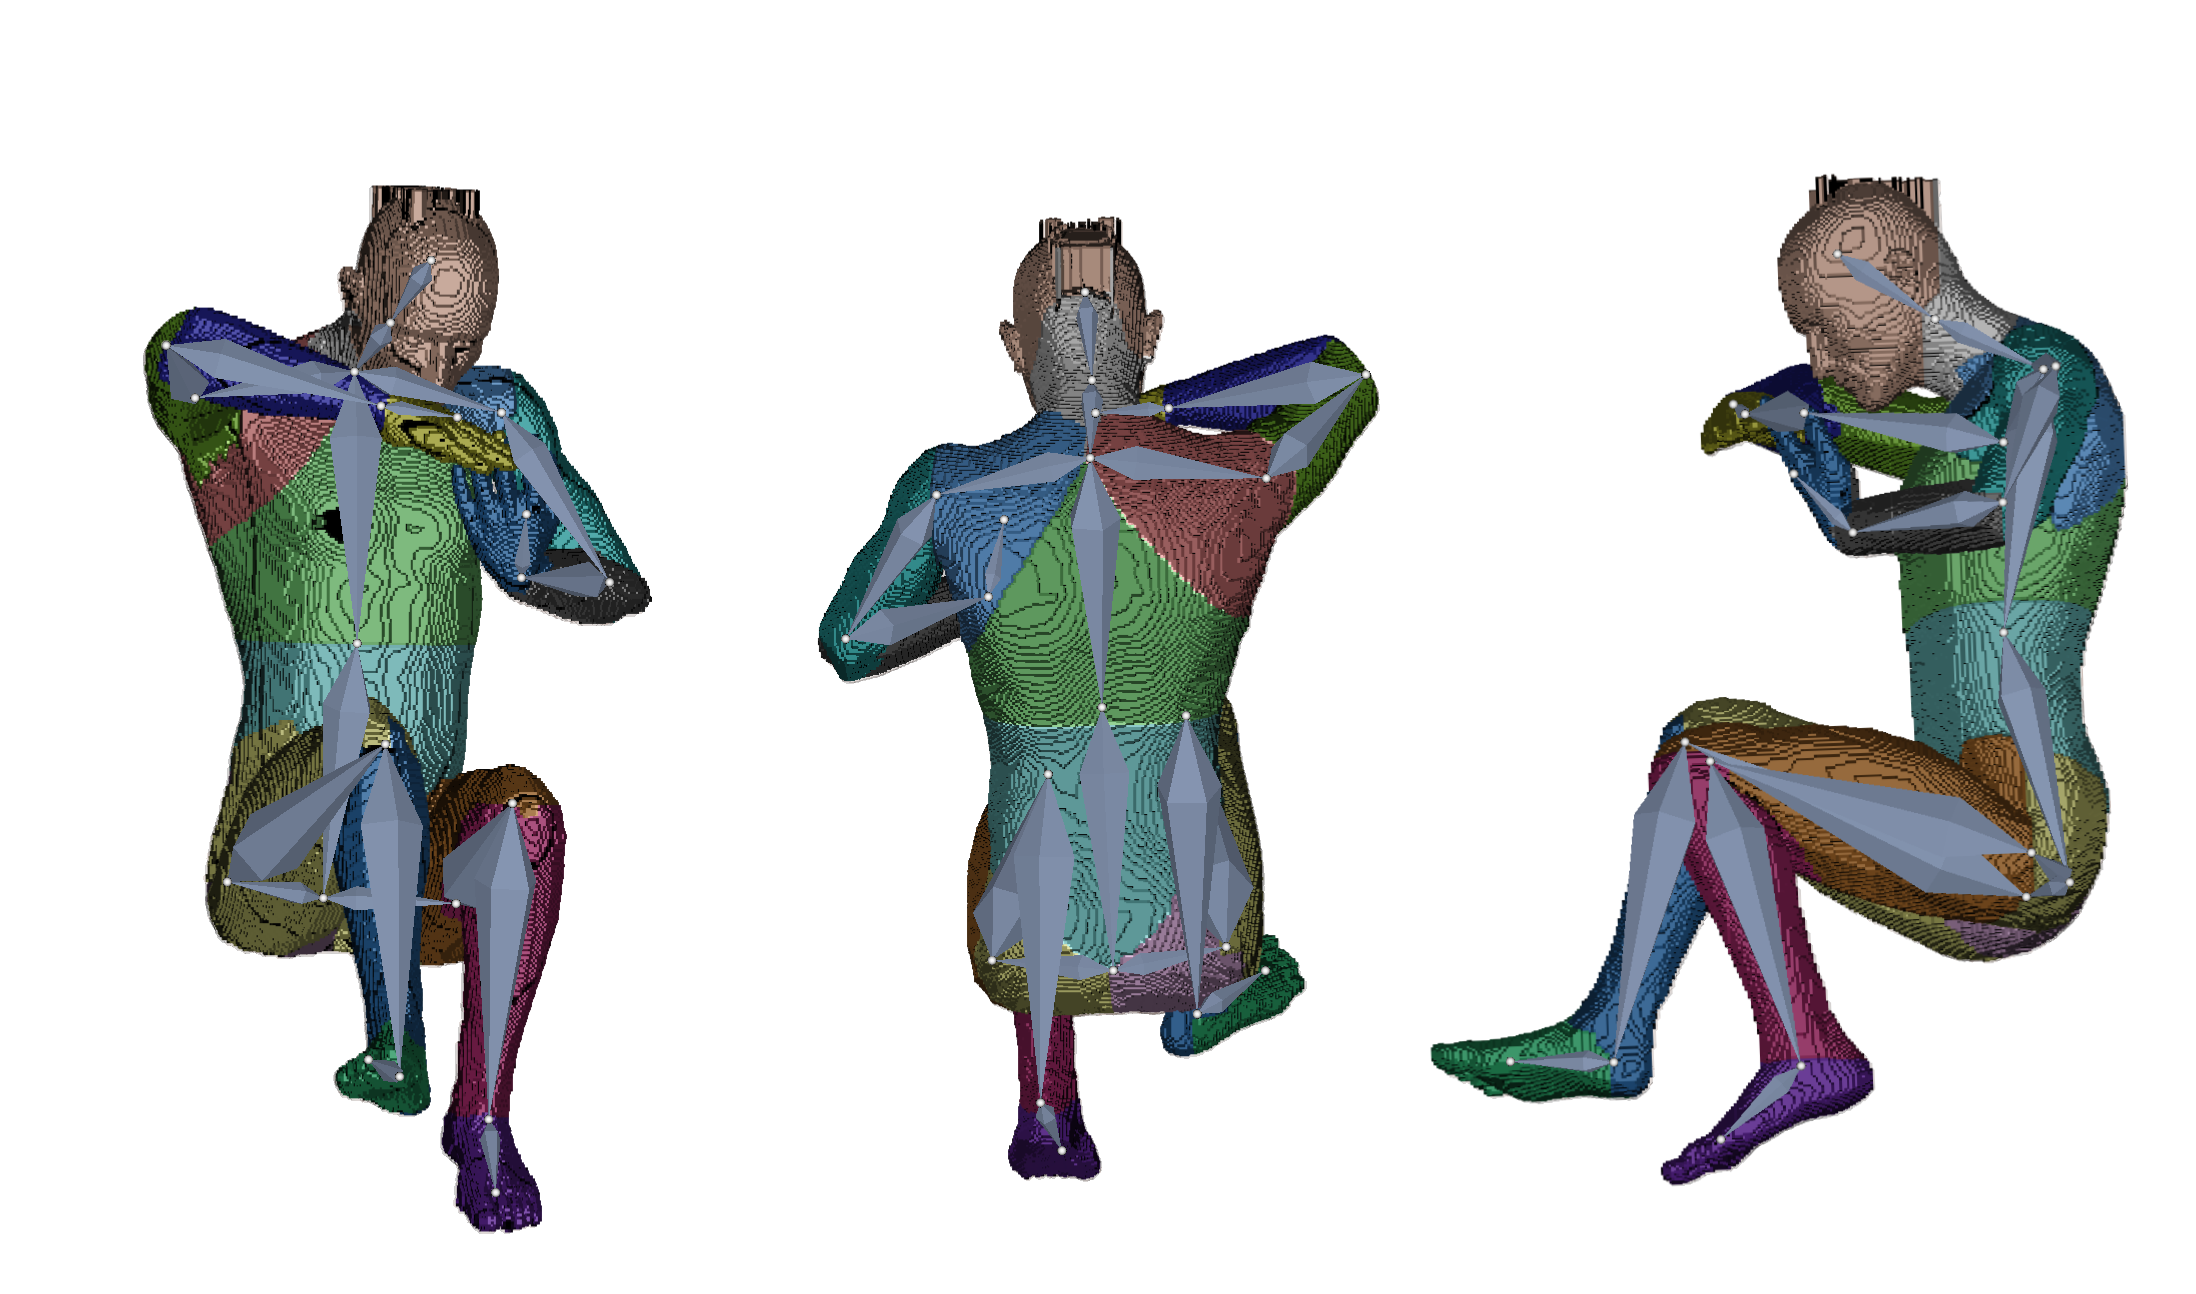
\includegraphics[width=12cm]{content/images/weight}
	\caption{Result of the weighting module in Bender. The colors represent the mapping to the according segments of the armature inside of the volume.} 
	\label{fig:weight}
\end{figure}


\newpage
\section{Transformation of the data}\label{sec:transformation}

The transformation of the data based on a model is the key feature introduced in this thesis. The transformation is done in 3D Slicer \cite{Slicer3DSlicer, Fedorov20123DNetwork} in an own extension with several modules that carry out the different operations needed in order to transform the data. The extension is portable and can be used for other purposes as well.

\subsection{Loading model and armature}

The first step of the processing in this module is to load the data as well as the armature. The armature is saved as *.vtk which is an own file format of the \gls{vtk}. It represents the armature as a graph which consists of several segments. Each segment is defined by an unique identifier and the segments are given by coordinates which state where the head and the tail of the segment is located in the coordinate system in \gls{3d}. The segments are always connected by their head except the first segment. The volumetric data is given in another file format namely *.mha which is a so called Meta Image. This file format is specified by the \gls{itk} and it contains the volumetric data. The input to this module is more specifically the output of the prior used Bender application which already includes the affiliation of the voxels to the segments of the armature by setting their value to the identifier of the segments of the armature. The data might be visualized using the $VolumeRendering$ module of the 3D slicer. Using it also reveals the mapping between the voxels and the amateur. A visualization of an example output may be seen in Figure \ref{fig:volumeRendering}.


\begin{figure} [!htb]
    \centering
	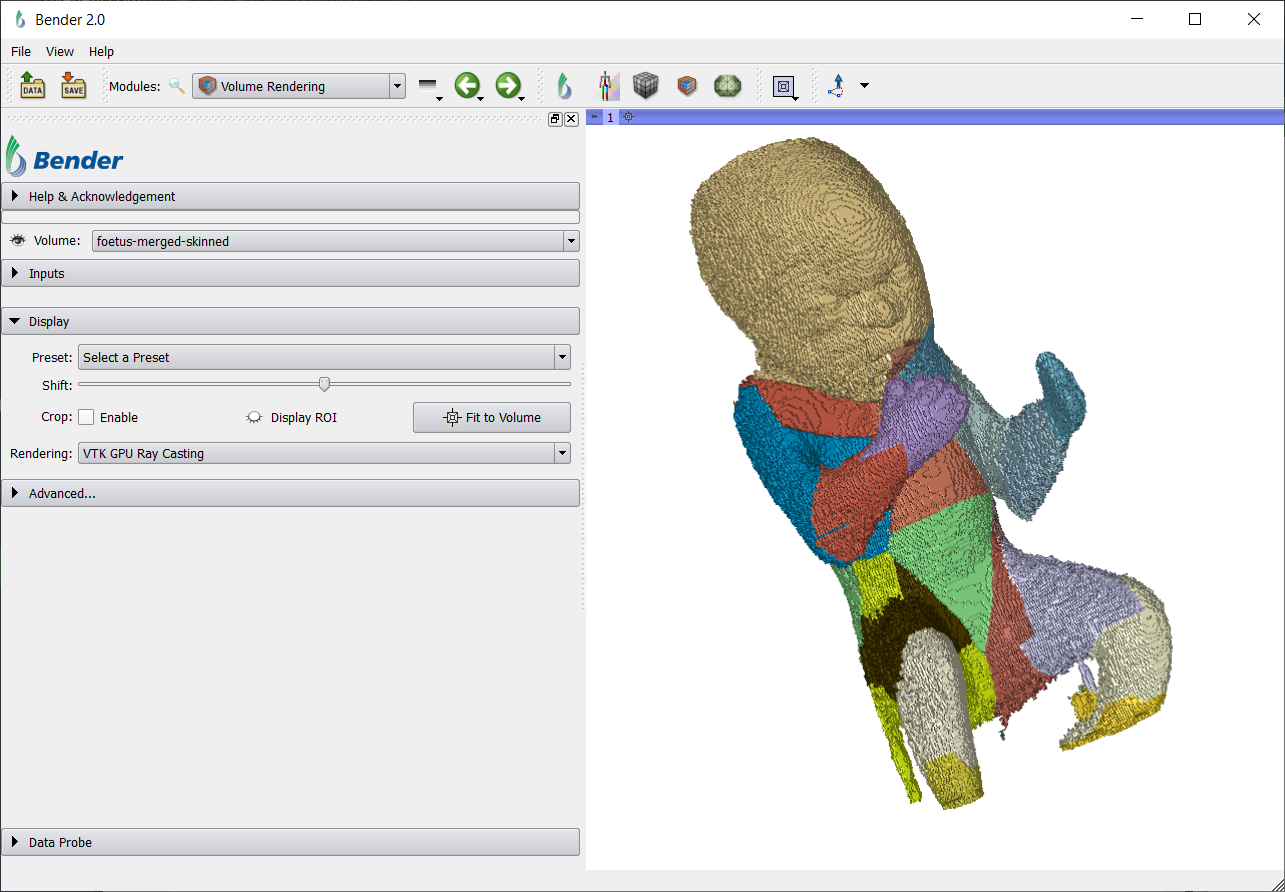
\includegraphics[width=8cm]{content/images/volumeRendering}
	\caption{Output of the $VolumeRendering$ module of 3D Slicer when visualizing the weighted fetus phantom model.} 
	\label{fig:volumeRendering}
\end{figure}


\newpage
\subsection{Calculate transform for each segment}

The basic idea of the approach is to transform each segment of the armature in respect to the segment attached or in some special cases like the transformation of the legs in respect to another segment which is not connected. The transformation that is needed is calculated by thinking of rotating the segment in a way, that it faces into the same direction then the segment before. In order to visualize this transformation process the left arm of a phantom is used. In this example the forearm of the left hand shall be transformed in a way that it faces in the same direction than the left upper arm. The left hand is just visualized in order to make the arm situation better perceivable. Of course the left arm also has to be transformed in order to align with the left forearm. The visualization of the initial pose is depicted in Figure \ref{fig:leftArm}.The legs are a somehow special case, because they should point in the same direction as the spine does and not as the abstraction of the pelvis does.

\begin{figure} [!htb]
    \centering
	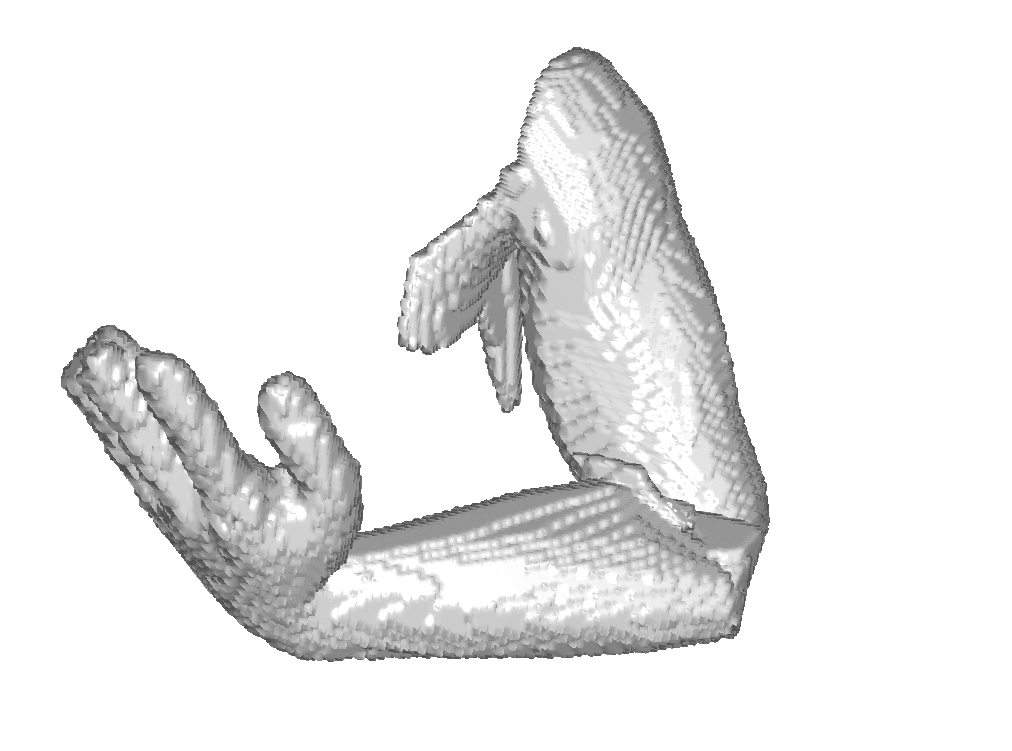
\includegraphics[width=10cm]{content/images/leftArm}
	\caption{Visualization of the initial pose of the left arm before transforming it.} 
	\label{fig:leftArm}
\end{figure}

In order to make the problem definition perceivable from a mathematical view the forearm is shifted to the head of the left upper arm. This represents a positioning of the coordinate system to the head of the left upper arm and shifting the left forearm to the origin of the new coordinate system. This does not have to be done in that way during the implementation it is only a way to visualize the methodical approach presented in this work.

\begin{figure} [!htb]
    \centering
	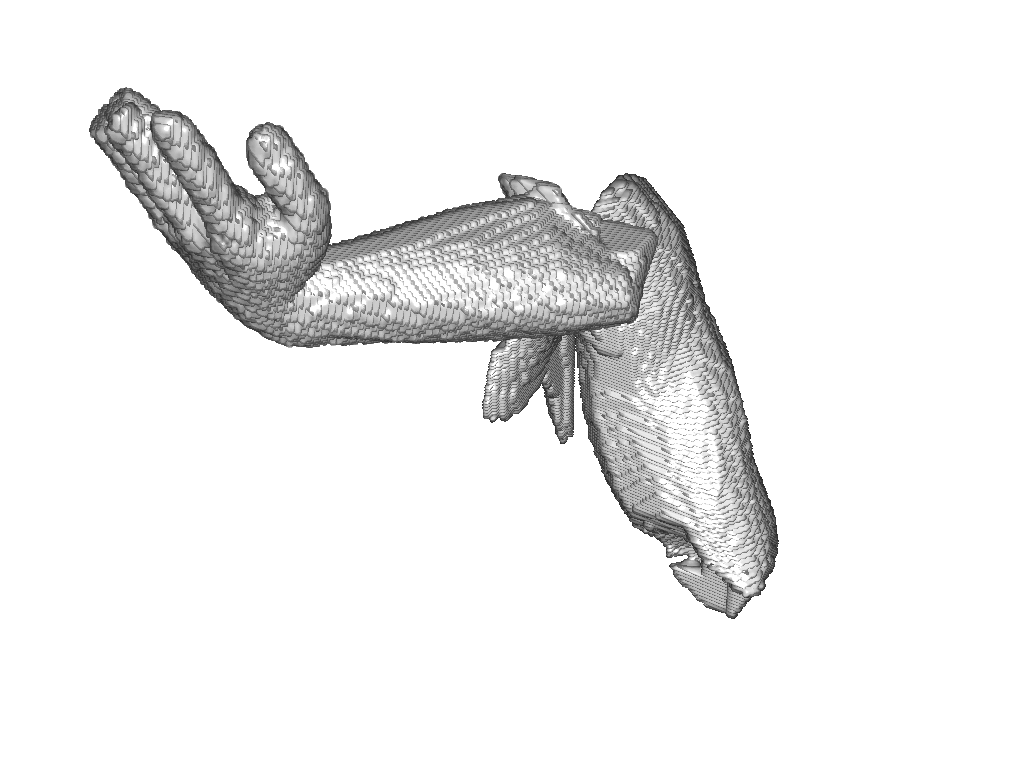
\includegraphics[width=10cm]{content/images/coordinateSystemShift}
	\caption{Image of the left forearm and hand shifted to the origin of the left upper arm in order to visualize the coordinate system shift.} 
	\label{fig:coordinateSystemShift}
\end{figure}

\newpage
\subsubsection{Mathematical basis}

For better understanding the problem is visualized as two vectors using Matlab. Figure \ref{fig:matlab} represents the output of the vector visualization. 

\begin{figure} [!htb]
    \centering
	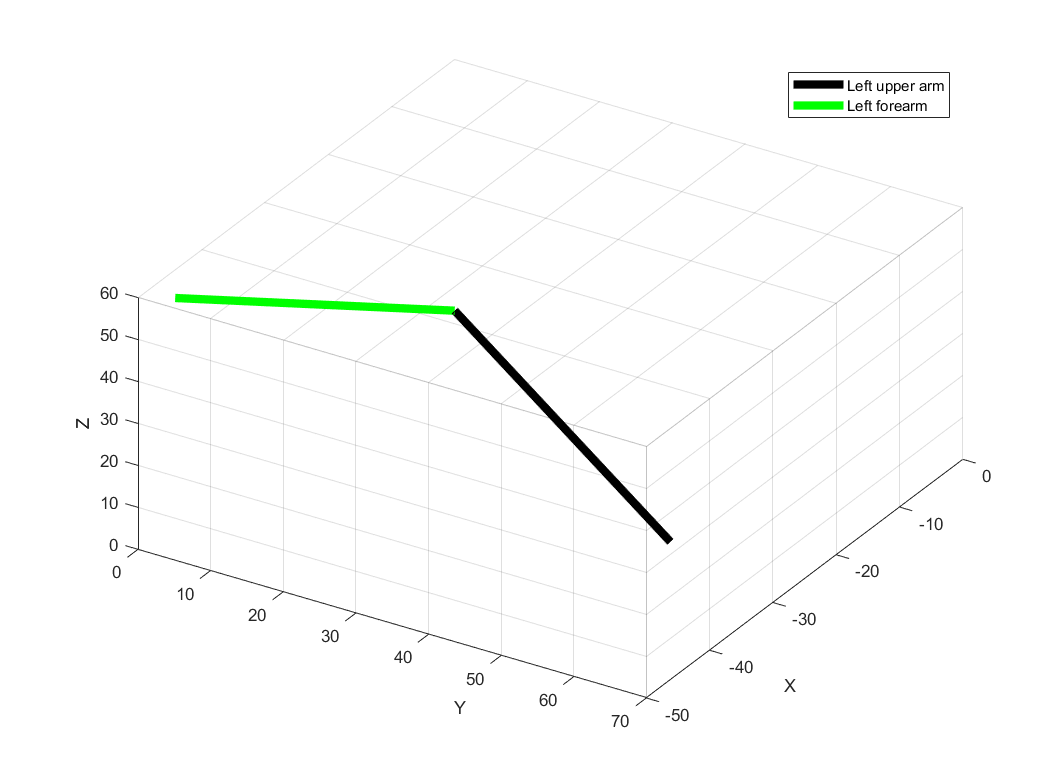
\includegraphics[width=10cm]{content/images/matlab.png}
	\caption{Vector representation of the left arm in Matlab, black being the left upper arm and green the left forearm.} 
	\label{fig:matlab}
\end{figure}

The result of the transformation for most of the segments should be that they face directly in the same direction. To do so two calculations have to be done. First an axis of rotation has to be found and second the angle between the two vectors. The angle of rotation is calculated by the Equation \ref{eq:axis} where u and v are the two vectors and a is the axis of rotation.

\begin{equation}
    a = u \times v / ||u \times v ||
    \caption{Axis of rotation between two vectors}
    \label{eq:axis}
\end{equation}

The angle between the vectors is calculated by Equation \ref{eq:angle}

\begin{equation}
    \alpha = arccos(u \cdot v)
    \caption{Angle between two vectors}
    \label{eq:angle}
\end{equation}

Having this information given one can easily calculate the rotation matrix about this arbitrary axis using the information provided my McDonald in his paper \cite{McdonaldAnimatedAxis}. Before representing the rotation matrix two further definitions have to be made, namely $c = cos(\alpha)$ and $s = sin(\alpha)$. The rotation matrix is presented in Equation \ref{eq:Rotation}.

\begin{equation}
    M_r = 
    \begin{bmatrix} 
    a_x^2(1-c)+c     & a_xa_y(1-c)-a_zs & a_xa_z(1-c)+a_ys \\
    a_xa_y(1-c)+a_zs & a_y^2(1-c)+c     & a_ya_z(1-c)-a_xs \\
    a_xa_z(1-c)-a_y  & a_ya_z(1-c)+a_xs & a_z^2(1-c)+c    
    \end{bmatrix} 
    \caption{Rotation matrix for rotation about an arbitrary axis \cite{McdonaldAnimatedAxis}.}
    \label{eq:RotationMatrix}
\end{equation}

McDonald states in his paper that it is important to have a as a unit vector because the matrix would not represent a rotation if it is not. The fact is that the rotation would be multiplied with the angle of rotation and therefore the result would not be the desired one. In Equation \ref{eq:Rotation} the result of the operation is shown in order to rotate a vector in the same direction than another one.

\begin{equation}
    v_r = M_ru
    \caption{Rotation of a vector in the direction of another vector by applying a rotation matrix about an arbitrary axis.}
    \label{eq:Rotation}
\end{equation}

Applying the rotation matrix to the given example the two vectors finally look like presented in the Figure \ref{fig:matlab2}.

\begin{figure} [!htb]
    \centering
	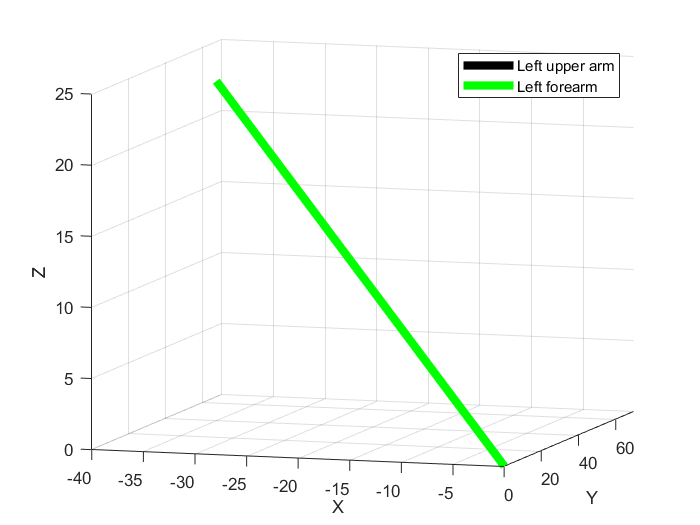
\includegraphics[width=10cm]{content/images/matlab2}
	\caption{Visualisation of the rotation result in Matlab. The black and the green vector representing the forearm and the upper arm are perfectly aligned.} 
	\label{fig:matlab2}
\end{figure}

The result in terms of data can be seen in Figure \ref{fig:leftArmOrRotation}. It represents the left forearm rotated in direction of the left upper arm. The whole rotation is then carried out without moving the forearm to the head of the upper arm. Instead the center of rotation is at the head of the forearm which is in fact the connection point between those two segments.The result of the rotation in that point is depicted in Figure \ref{fig:leftArmRRotation}.

\begin{figure} [!htb]
    \centering
	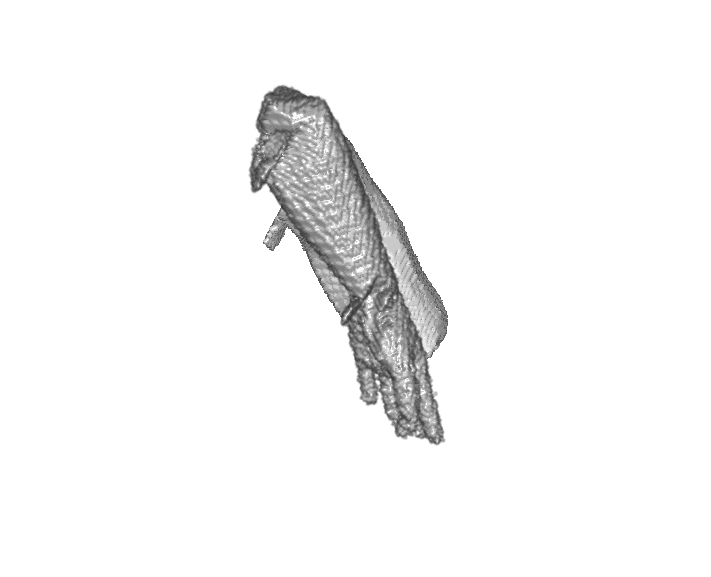
\includegraphics[width=10cm]{content/images/leftArmOrRotation.png}
	\caption{Result of the rotation of the left forearm with the center of rotation at the head of the left upper arm. Of course the left forearm has been moved to this point before.} 
	\label{fig:leftArmOrRotation}
\end{figure}
\begin{figure} [!htb]
    \centering
	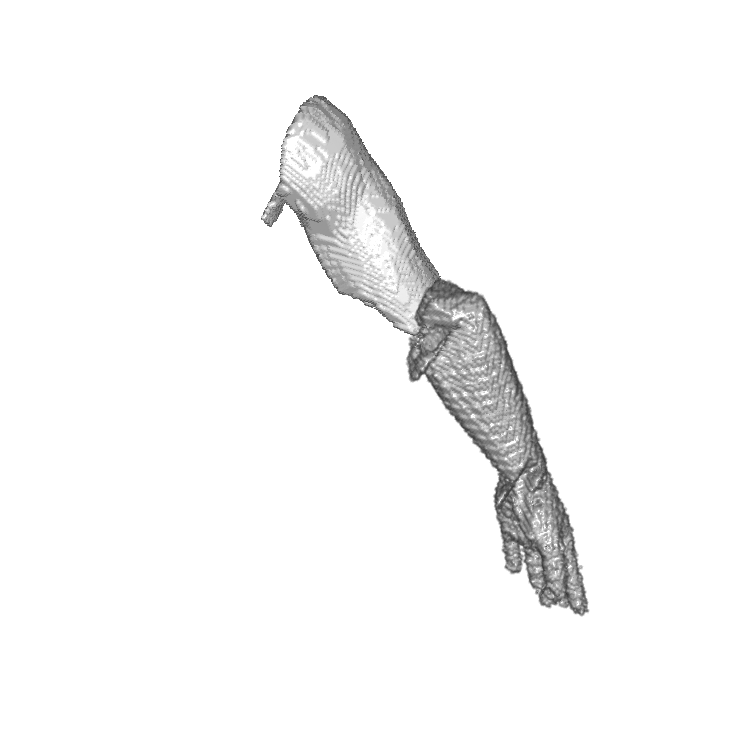
\includegraphics[width=10cm]{content/images/leftArmRRotation.png}
	\caption{Result of the rotation of the left forearm with the center of rotation at the connection point between left forearm and left upper arm.} 
	\label{fig:leftArmRRotation}
\end{figure}

\newpage
\subsection{Apply transform}

Having the rotation matrix defined which rotates one segment in the direction of the other segment the next step is to apply this transform to the voxels which belong to it. There is also one detail which should be kept in mind. The rotation matrix only describes the rotation around the arbitrary axis but the origin of the axis has to be set to be at the joint between two segments. This step may be performed by first shifting the segment of interest to the origin of the coordinate system, apply the transform there and shift it back. Or another possibility is to apply the transform considering a specific center of rotation. Some transformations are able to take such a center into account.

\newpage
\subsubsection{Integration in visualization framework}
In context of working with \gls{3d} visualization \gls{itk} is well known. Therefore we decided to work with it in terms of applying the transformation. The transformation is based on a given matrix and the center of rotation. Having both information the transformation is simply applied at the data using a $Resample$ filter. The filter takes the original image and the transformation an creates the output volume.\newline

\subsection{Save output}
The output of the method can be described as a volume which is a collection of volumes which represents the different parts of the armature. The volume can be saved as one file but the information about all the segments is also available. So for instance if one would like to examine the hand or the forearm of the fetus in greater detail there would also be the possibility to save those separately. In this work the save functionality of 3D Slicer is used which may be found in the Menu of the program. A screenshot of the program is depicted in Figure \ref{fig:saving}.


\begin{figure} [!htb]
    \centering
	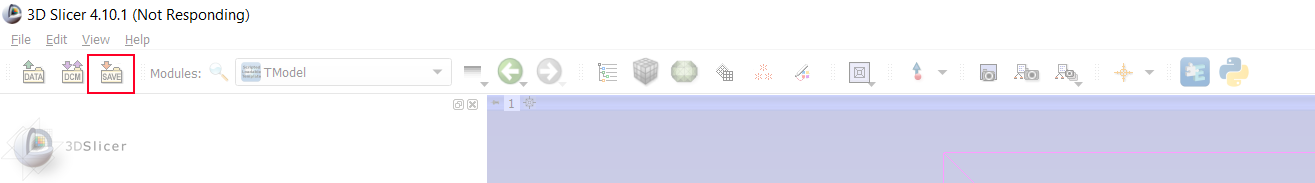
\includegraphics[width=12cm]{content/images/saving.png}
	\caption{Saving option in the menu of 3D Slicer.} 
	\label{fig:saving}
\end{figure}

\section{Analysis}
The analysis of data may be performed in many different ways. There could be of course some automatically performed analysis steps which may be performed on the generated output data. Those could for example calculate or display the range of the volumetric data in all three dimensions. This would then correlate to the crown toe distance and the spread of the arms. Normally one would measure these parameters by viewing at a \gls{2d} slice of the ultrasound like described in \ref{subsct:fetalGrowth}. Due to the fact that the method analysis and transforms each segment separately the volumetric information of each part is already given for analysis. So if it is needed there could be also volumetric statistics applied like how much volume does the head or some other parts of the body have. It can even be automatically compared if the volume of the right or the left limb is significantly higher. This would maybe the case in some growth disorders.

\newpage
In this work automatically analysis of the output data is not performed but there is a way to take measurements manually. 3D Slicer provides the user with a set of analysis tools like a ruler. The ruler can be applied in the 3D view and delivers the exact distance between two points. If the ruler is applied at the crown and the toe it will deliver the crown toe distance. Another more common distance would be the crown rump measurement. In Figure \ref{fig:ruler} the ruler can be seen in the toolbar and in Figure \ref{fig:rulerResult} the visualization in the 3D view of Slicer is shown. The ruling is performed interactively and can be adapted in the \gls{3d} view.\newline


\begin{figure} [!htb]
    \centering
	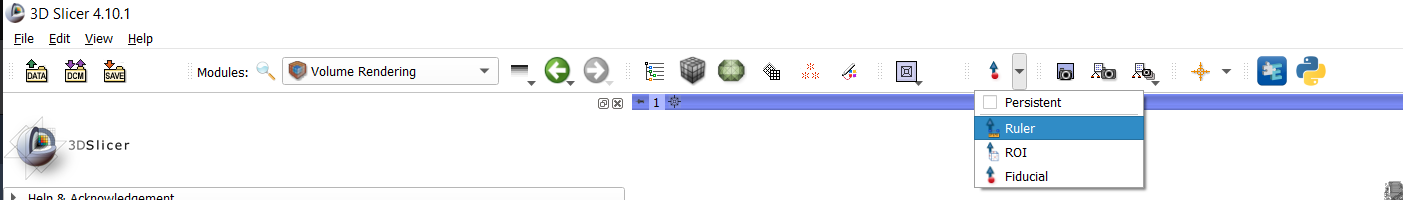
\includegraphics[width=14cm]{content/images/ruler.png}
	\caption{Ruler option in the 3D Slicer menu.} 
	\label{fig:ruler}
\end{figure}

\begin{figure} [!htb]
    \centering
	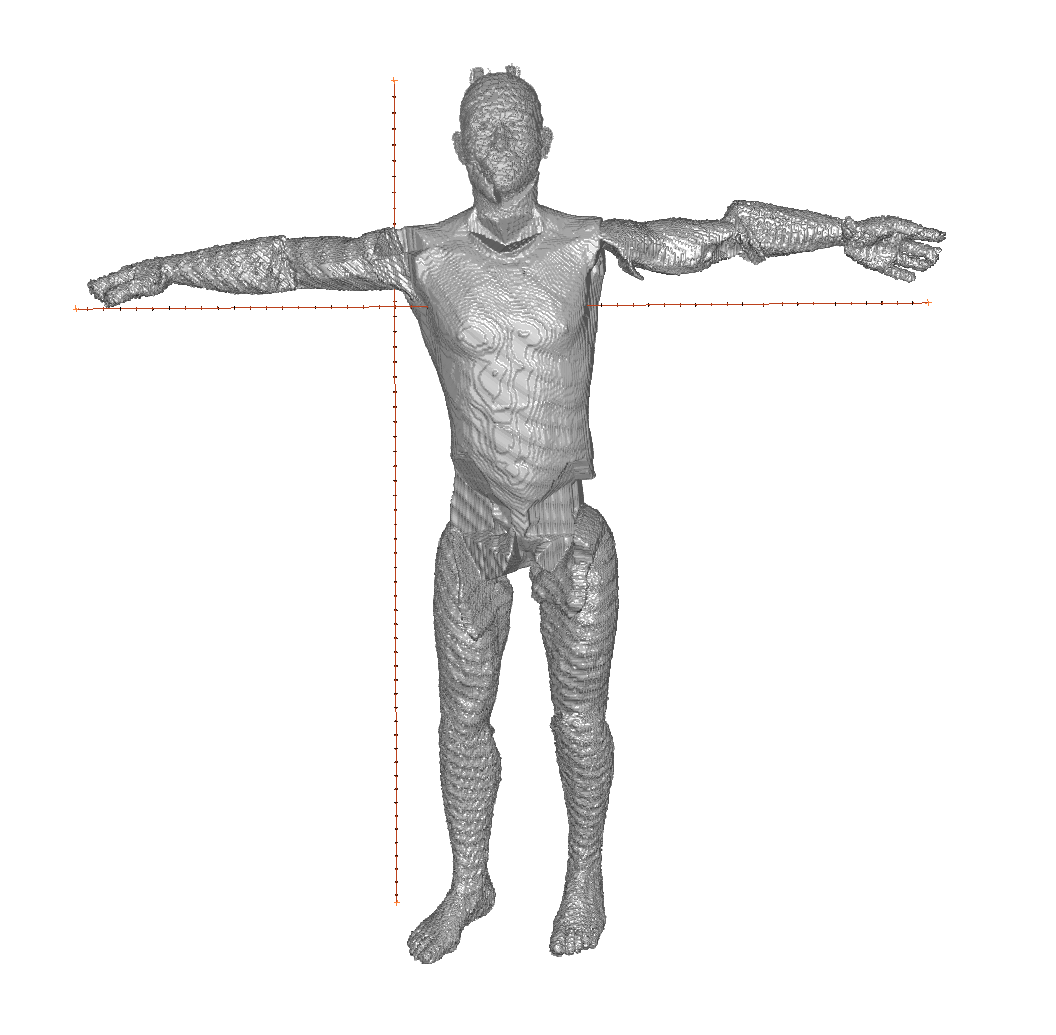
\includegraphics[width=16cm]{content/images/rulerResult.png}
	\caption{Result of two ruler operations on the T transformed model measuring the crown toe length and the spread of the arms.} 
	\label{fig:rulerResult}
\end{figure}